% This LaTeX was auto-generated from MATLAB code.
% To make changes, update the MATLAB code and export to LaTeX again.

\documentclass{article}

\usepackage[utf8]{inputenc}
\usepackage[T1]{fontenc}
\usepackage{lmodern}
\usepackage{graphicx}
\usepackage{color}
\usepackage{listings}
\usepackage{hyperref}
\usepackage{amsmath}
\usepackage{amsfonts}
\usepackage{epstopdf}
\usepackage{matlab}

\sloppy
\epstopdfsetup{outdir=./}
\graphicspath{ {./locating_a_moving_target_sol_images/} }

\begin{document}

\matlabtitle{2. Locating a moving target}


\matlabheading{2.0 Initialization}

\begin{matlabcode}
clear;
\end{matlabcode}


\matlabheading{2.1 The setup}



\matlabheading{2.2 Distance from a critical point (Example)}

\begin{matlabcode}
% Given data
t_k = [0 1 1.5 3 4.5];
c_k = [-1.7210 -4.3454; 1.0550 -3.0293; 2.9619 -1.5857; 3.8476 1.2253; 7.1086 4.9975]';
R_k = [0.9993 1.4618 2.2617 1.0614 1.6983];
t_star = 8;
x_star = [6;10];

cvx_begin quiet
    % optimization variables
    variables p0(2,1) v(2,1)
    % cost function
    minimize(norm(p0+t_star*v-x_star));
    % subject to
    for k = 1:length(t_k)
        norm(p0+t_k(k)*v-c_k(:,k)) <= R_k(k);
    end
cvx_end

p_k = p0+kron([t_k t_star],v); 
minimumDistance = norm(p0+t_star*v-x_star);

% ---------- Plot result ----------
% trajectory
figure('units','normalized','outerposition',[0 0 1 1]);
hold on;
set(gca,'FontSize',35);
ax = gca;
ax.XGrid = 'on';
ax.YGrid = 'on';
axis equal;
title('2.2 Distance from critical point (example)');
theta = 0:0.01:2*pi;
for k = 1:length(t_k)
    p = plot(R_k(k)*cos(theta)+c_k(1,k),R_k(k)*sin(theta)+c_k(2,k),'Color','blue');
    p.LineWidth = 3;
    text(c_k(1,k),c_k(2,k),sprintf('%d',k),'FontSize',25,'HorizontalAlignment', 'center');
end
scatter(p_k(1,:),p_k(2,:),300,'s','red','LineWidth',4);
scatter(x_star(1),x_star(2),300,'o','MarkerFaceColor','black');
text(x_star(1)-0.75,x_star(2)-0.75,'$x^{\star}$','Interpreter','latex','FontSize',35,'HorizontalAlignment', 'center');
ylabel('$p_y$','Interpreter','latex');
xlabel('$p_x$','Interpreter','latex');
saveas(gcf,'./locating_a_moving_target_data/2_2_example.fig');
saveas(gcf,'./locating_a_moving_target_data/2_2_example.png');
hold off;
\end{matlabcode}
\begin{center}
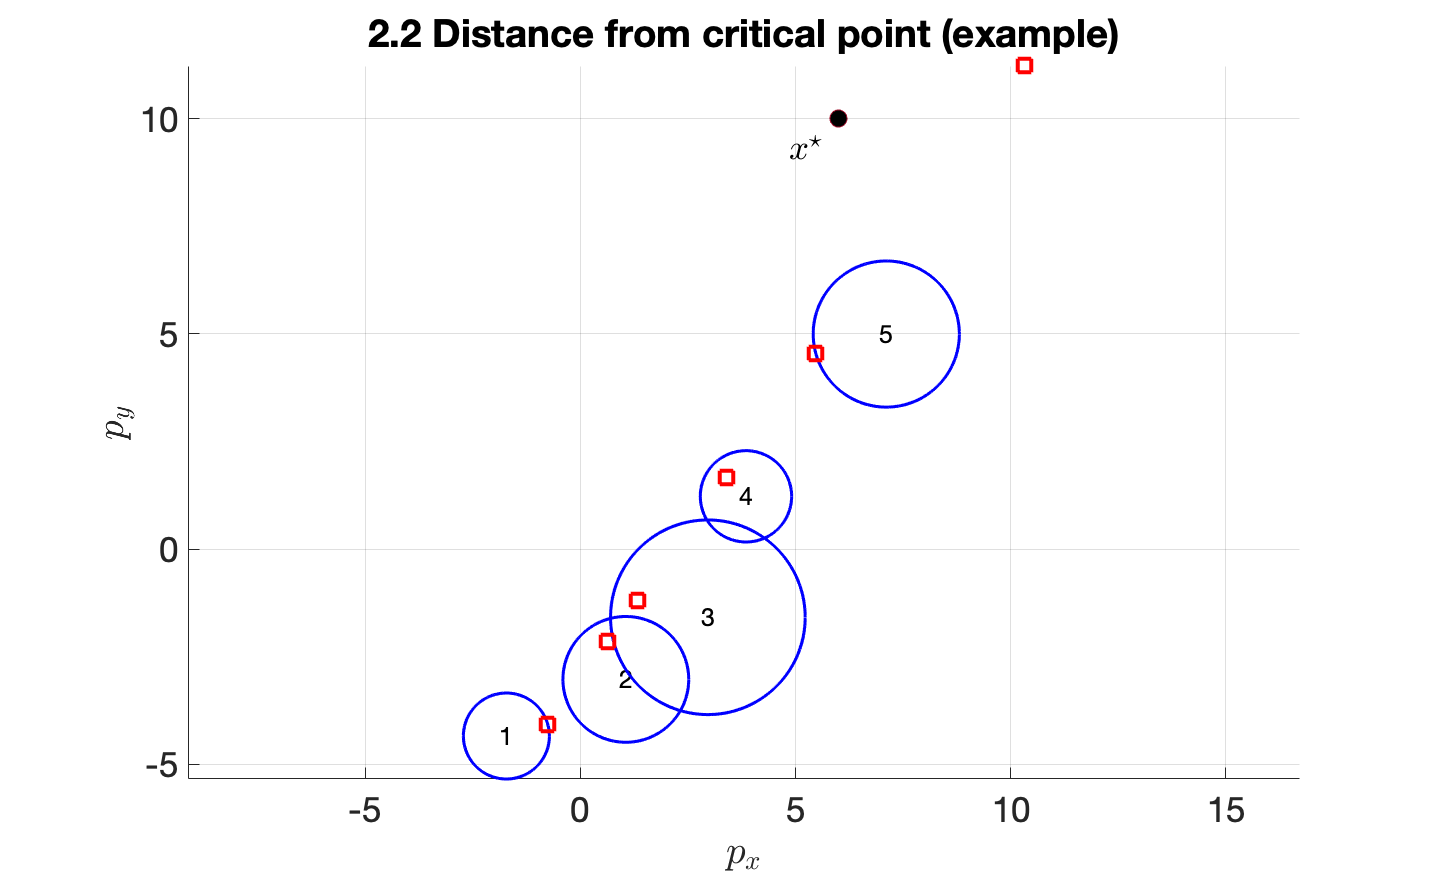
\includegraphics[width=\maxwidth{144.5057701956849em}]{figure_0}
\end{center}
\begin{matlabcode}

fprintf("The minimum distance to x_star at t_star is %f with: \n",minimumDistance);
\end{matlabcode}
\begin{matlaboutput}
The minimum distance to x_star at t_star is 4.494781 with: 
\end{matlaboutput}
\begin{matlabcode}
p0
\end{matlabcode}
\begin{matlaboutput}
p0 = 2x1    
   -0.7597
   -4.0725

\end{matlaboutput}
\begin{matlabcode}
v
\end{matlabcode}
\begin{matlaboutput}
v = 2x1    
    1.3855
    1.9125

\end{matlaboutput}
\begin{matlabcode}
save('./locating_a_moving_target_data/2_2_data_example.mat','minimumDistance','p0','v');
\end{matlabcode}


\matlabheading{2.2 Distance from a critical point}

\begin{matlabcode}
% Given data
t_k = [0 1 1.5 3 4.5];
c_k = [0.6332 -3.2012; -0.0054 -1.7104; 2.3322 -0.7620; 4.4526 3.1001; 6.1752 4.2391]';
R_k = [2.2727 0.7281 1.3851 1.8191 1.0895];
t_star = 8;
x_star = [6;10];

\end{matlabcode}

\begin{par}
\begin{flushleft}
The initial position $\mathbf{p}_0$ and velocity $\mathbf{v}$are unknown but the model of the movement of the target is: $\mathbf{p}(t) = \mathbf{p}_0+t\mathbf{v}$. The only information given about the position of the target are the discs where the target was located at a given point in time. So these are the constarint of the otimization problem. Given that it is impossible to determine  the initial position $\mathbf{p}_0$ and velocity $\mathbf{v}$ based on the disc information (unless if the discs are colinear and of null radius) we would like to find the worst case possible, i.e., the initial position $\mathbf{p}_0$ and velocity $\mathbf{v}$ such that, knowing the disc information, allows for the target to be the closest to $\mathbf{x}^{\star}$at $t^{\star}$. For that reason the optimization problem is
\end{flushleft}
\end{par}

\begin{par}
\begin{flushleft}
$\min_{\mathbf{p}_0,\mathbf{v}} \quad ||\mathbf{p}_0+t^{\star}\mathbf{v}-\mathbf{x}^{\star}||_2 \quad \mathrm{subject\;to} \quad ||\mathbf{p}_0+t_k\mathbf{v}-\mathbf{x}_k||_2 \leq R_k, \; k = 1,\ldots,K$.
\end{flushleft}
\end{par}

\begin{matlabcode}

cvx_begin quiet
    % optimization variables
    variables p0(2,1) v(2,1)
    % cost function
    minimize(norm(p0+t_star*v-x_star));
    % subject to
    for k = 1:length(t_k)
        norm(p0+t_k(k)*v-c_k(:,k)) <= R_k(k);
    end
cvx_end

p_k = p0+kron([t_k t_star],v); 
minimumDistance = norm(p0+t_star*v-x_star);

% ---------- Plot result ----------
% trajectory
figure('units','normalized','outerposition',[0 0 1 1]);
hold on;
set(gca,'FontSize',35);
ax = gca;
ax.XGrid = 'on';
ax.YGrid = 'on';
axis equal;
title('2.2 Distance from critical point');
theta = 0:0.01:2*pi;
for k = 1:length(t_k)
    p = plot(R_k(k)*cos(theta)+c_k(1,k),R_k(k)*sin(theta)+c_k(2,k),'Color','blue');
    p.LineWidth = 3;
    text(c_k(1,k),c_k(2,k),sprintf('%d',k),'FontSize',25,'HorizontalAlignment', 'center');
end
scatter(p_k(1,:),p_k(2,:),300,'s','red','LineWidth',4);
scatter(x_star(1),x_star(2),300,'o','MarkerFaceColor','black');
text(x_star(1)-0.75,x_star(2)-0.75,'$x^{\star}$','Interpreter','latex','FontSize',35,'HorizontalAlignment', 'center');
ylabel('$p_y$','Interpreter','latex');
xlabel('$p_x$','Interpreter','latex');
saveas(gcf,'./locating_a_moving_target_data/2_2.fig');
saveas(gcf,'./locating_a_moving_target_data/2_2.png');
hold off;
\end{matlabcode}
\begin{center}
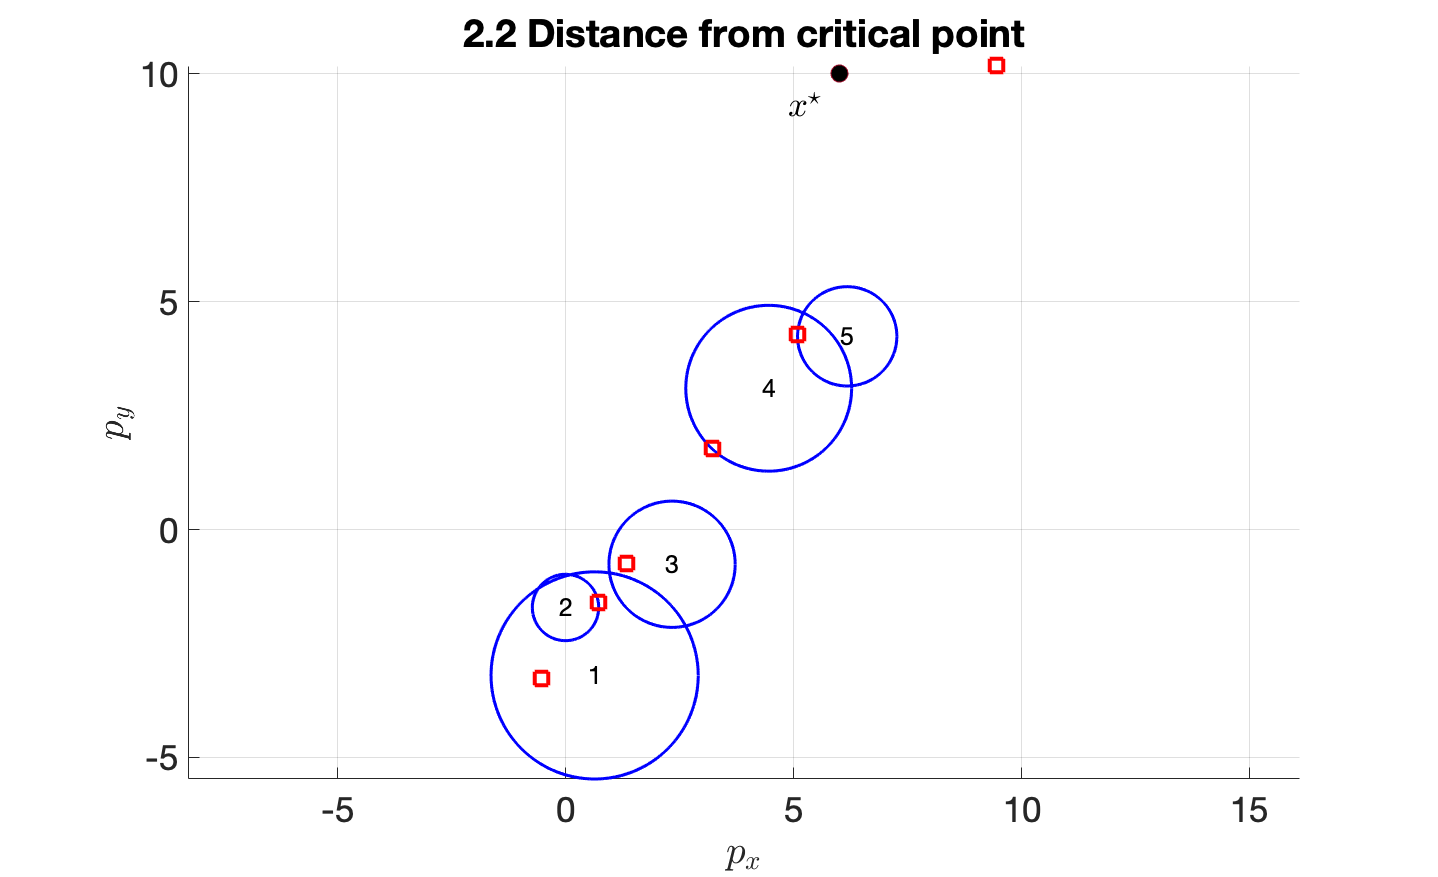
\includegraphics[width=\maxwidth{144.5057701956849em}]{figure_1}
\end{center}
\begin{matlabcode}

fprintf("The minimum distance to x_star at t_star is %f with: \n",minimumDistance);
\end{matlabcode}
\begin{matlaboutput}
The minimum distance to x_star at t_star is 3.465101 with: 
\end{matlaboutput}
\begin{matlabcode}
p0
\end{matlabcode}
\begin{matlaboutput}
p0 = 2x1    
   -0.5368
   -3.2715

\end{matlaboutput}
\begin{matlabcode}
v
\end{matlabcode}
\begin{matlaboutput}
v = 2x1    
    1.2497
    1.6803

\end{matlaboutput}
\begin{matlabcode}
save('./locating_a_moving_target_data/2_2_data.mat','minimumDistance','p0','v');

\end{matlabcode}


\matlabheading{2.3 Smallest enclosing rectangle}

\begin{matlabcode}
% Given data
t_k = [0 1 1.5 3 4.5];
c_k = [0.6332 -3.2012; -0.0054 -1.7104; 2.3322 -0.7620; 4.4526 3.1001; 6.1752 4.2391]';
R_k = [2.2727 0.7281 1.3851 1.8191 1.0895];
t_star = 8;
\end{matlabcode}

\begin{par}
\begin{flushleft}
The initial position $\mathbf{p}_0$ and velocity $\mathbf{v}$are unknown but the model of the movement of the target is: $\mathbf{p}(t) = \mathbf{p}_0+t\mathbf{v}$. The only information given about the position of the target are the discs where the target was located at a given point in time. So these are the constarint of the otimization problem. Given that it is impossible to determine  the initial position $\mathbf{p}_0$ and velocity $\mathbf{v}$ based on the disc information (unless if the discs are colinear and of null radius) we would like to find the worst case possible for each of the 4 main directions in the plane to find $a_1,a_2,b_1$ and $b_2$. Therefore, the solution to this task is found solving four independent optimization problems:
\end{flushleft}
\end{par}

\begin{par}
\begin{flushleft}
To find:
\end{flushleft}
\end{par}

\begin{itemize}
\setlength{\itemsep}{-1ex}
   \item{\begin{flushleft} $a_1$ solve  $\min_{\mathbf{p}_0,\mathbf{v}} \quad [1\;\;0](\mathbf{p}_0+t^{\star}\mathbf{v}) \quad \mathrm{subject\;to} \quad ||\mathbf{p}_0+t_k\mathbf{v}-\mathbf{x}_k||_2 \leq R_k, \; k = 1,\ldots,K$  and then assign $a_1 = [1\;\;0](\mathbf{p}_0+t^{\star}\mathbf{v})$; \end{flushleft}}
   \item{\begin{flushleft} $a_2$ solve  $\min_{\mathbf{p}_0,\mathbf{v}} \quad -[1\;\;0](\mathbf{p}_0+t^{\star}\mathbf{v}) \quad \mathrm{subject\;to} \quad ||\mathbf{p}_0+t_k\mathbf{v}-\mathbf{x}_k||_2 \leq R_k, \; k = 1,\ldots,K$  and then assign $a_2 = [1\;\;0](\mathbf{p}_0+t^{\star}\mathbf{v})$; \end{flushleft}}
   \item{\begin{flushleft} $b_1$ solve  $\min_{\mathbf{p}_0,\mathbf{v}} \quad [0\;\;1](\mathbf{p}_0+t^{\star}\mathbf{v}) \quad \mathrm{subject\;to} \quad ||\mathbf{p}_0+t_k\mathbf{v}-\mathbf{x}_k||_2 \leq R_k, \; k = 1,\ldots,K$  and then assign $b_1 = [0\;\;1](\mathbf{p}_0+t^{\star}\mathbf{v})$; \end{flushleft}}
   \item{\begin{flushleft} $b_2$ solve  $\min_{\mathbf{p}_0,\mathbf{v}} \quad -[1\;\;0](\mathbf{p}_0+t^{\star}\mathbf{v}) \quad \mathrm{subject\;to} \quad ||\mathbf{p}_0+t_k\mathbf{v}-\mathbf{x}_k||_2 \leq R_k, \; k = 1,\ldots,K$  and then assign $b_2 = [0\;\;1](\mathbf{p}_0+t^{\star}\mathbf{v})$; \end{flushleft}}
\end{itemize}

\begin{matlabcode}
rectangleCorners = zeros(4,1);
for i = 1:4
    E = [~idivide(i-1,int32(2)) double(idivide(i-1,int32(2)))];
    cvx_begin quiet
        % optimization variables
        variables p0(2,1) v(2,1)
        % cost function
        minimize(-(-1)^(i)*E*(p0+t_star*v));
        % subject to
        for k = 1:length(t_k)
            norm(p0+t_k(k)*v-c_k(:,k)) <= R_k(k);
        end
    cvx_end
    rectangleCorners(i) = E*(p0+t_star*v);
end

% ---------- Plot result ----------
% trajectory
figure('units','normalized','outerposition',[0 0 1 1]);
hold on;
set(gca,'FontSize',35);
ax = gca;
ax.XGrid = 'on';
ax.YGrid = 'on';
axis equal;
title('2.3 Smallest enclosing rectangle');
theta = 0:0.01:2*pi;
for k = 1:length(t_k)
    p = plot(R_k(k)*cos(theta)+c_k(1,k),R_k(k)*sin(theta)+c_k(2,k),'Color','blue');
    p.LineWidth = 3;
    text(c_k(1,k),c_k(2,k),sprintf('%d',k),'FontSize',25,'HorizontalAlignment', 'center');
end
rectangle('Position',...
    [rectangleCorners([1 3],1)' rectangleCorners(2,1)-rectangleCorners(1,1) rectangleCorners(4,1)-rectangleCorners(3,1)],...
    'FaceColor',[225/255 225/255 225/255],'LineWidth',3,'LineStyle','--');
ylabel('$p_y$','Interpreter','latex');
xlabel('$p_x$','Interpreter','latex');
saveas(gcf,'./locating_a_moving_target_data/2_3.fig');
saveas(gcf,'./locating_a_moving_target_data/2_3.png');
hold off;
\end{matlabcode}
\begin{center}
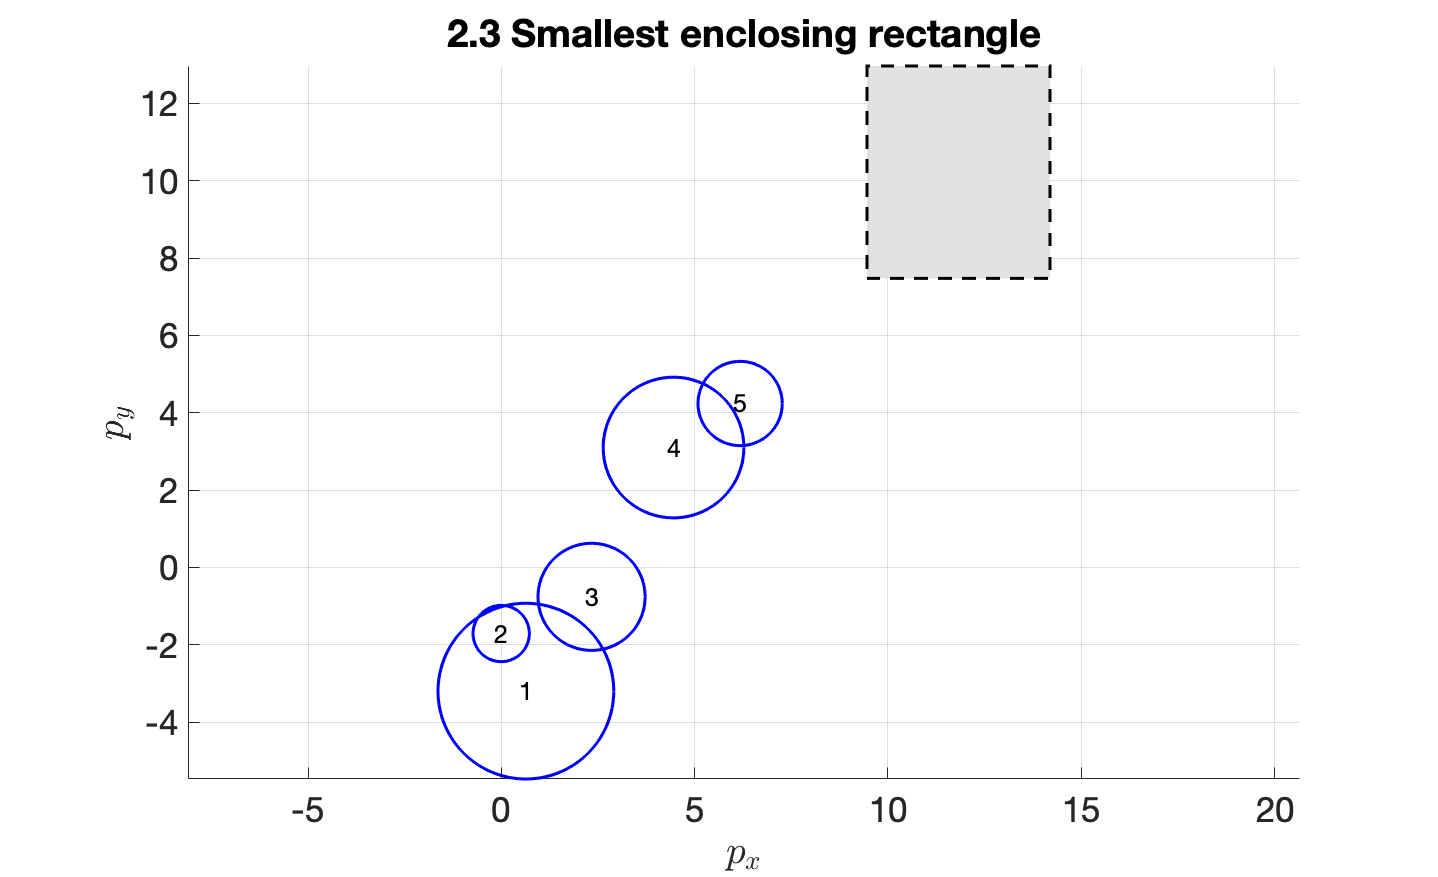
\includegraphics[width=\maxwidth{144.5057701956849em}]{figure_2}
\end{center}
\begin{matlabcode}

fprintf("The rectangle is defined by: a_1 = %f; a2 = %f; b1 = %f; b2 = %f.\n",...
    rectangleCorners(1,1),rectangleCorners(2,1),rectangleCorners(3,1),rectangleCorners(4,1));
\end{matlabcode}
\begin{matlaboutput}
The rectangle is defined by: a_1 = 9.458162; a2 = 14.190189; b1 = 7.476292; b2 = 12.969036.
\end{matlaboutput}
\begin{matlabcode}
save('./locating_a_moving_target_data/2_3_data.mat','rectangleCorners');



\end{matlabcode}

\end{document}
